\begin{comment}
Describe what you expect to deliver:
• A working prototype or simulation
• Performance metrics (e.g., signal-to-noise ratio (SNR) improvement, Perceptual Evaluation
of Speech Quality (PESQ) score)
• GitHub documentation and demonstration
\end{comment}
\noindent
Of course, the ultimate deliverable will be a working prototype of picoDAW deployed onto the 
provided GitHub project site. Given the complexity of a DAW however---even a stripped down 
one, only a sequencer/synthesizer/sampler---the core mantra behind the project will be to 
keep it simple, stupid. 

This means, the UI will be basic without the polish of the actual 
DS-10 it'll take inspiration from. Furthermore, though audio effects like real-time reverb 
or delay, and features like a semi-modular patchbay, are incredibly useful in modern music 
creation, they will not be prioritised over a working prototype.

What is a non-negotiable 
though, is the inclusion of a low pass and high pass filter for each instrument, 
and an envelope to control its cutoff frequency; alongside a second envelope for volume. In summary,
the expected features will be a:
\begin{enumerate}
	\item Synthesizer and sampler as instruments
		\begin{itemize}
		\item 4 Synthesizers; each has sine, saw, triangle, square, and noise as possible oscillator options
		\item 2 Samplers; each can load a \texttt{.wav} sample from 0.1 to 1 second, resampled to 48kHz on upload
		\end{itemize}
	\item Step sequencer with 16 steps. At a default 120bpm, this means only 8 seconds of audio, played in a loop
		\begin{itemize}
		\item The 6 instruments will each have their own
		\item The sequencer will have two screens
			\begin{itemize}
			\item one for sequencing what key is pressed and when
			\item one for how long that key should be pressed
			\end{itemize}
		termed Note and Gate respectively on the DS-10
		\item Changes to pattern during play will reflect on loop
		\end{itemize}
	\item Filter with adjustable cutoff and peak/resonance, toggled between lowpass and highpass.
		\begin{itemize}
		\item The 6 instruments will each have their own filter
		\end{itemize}
	\item ADSR\footnote{\url{https://en.wikipedia.org/wiki/Envelope_(music)\#ADSR}} envelope
		\begin{itemize}
		\item The 6 instruments will each have two envelopes
			\begin{itemize}
			\item one for modulating the cutoff of its filter
			\item one for modulating the volume of its output
			\end{itemize}
		\end{itemize}
	\item Mixer
		\begin{itemize}
		\item Basic; toggle mute or solo for each instrument
		\end{itemize}
\end{enumerate}

\begin{figure}[!hbtp]
	\centering
	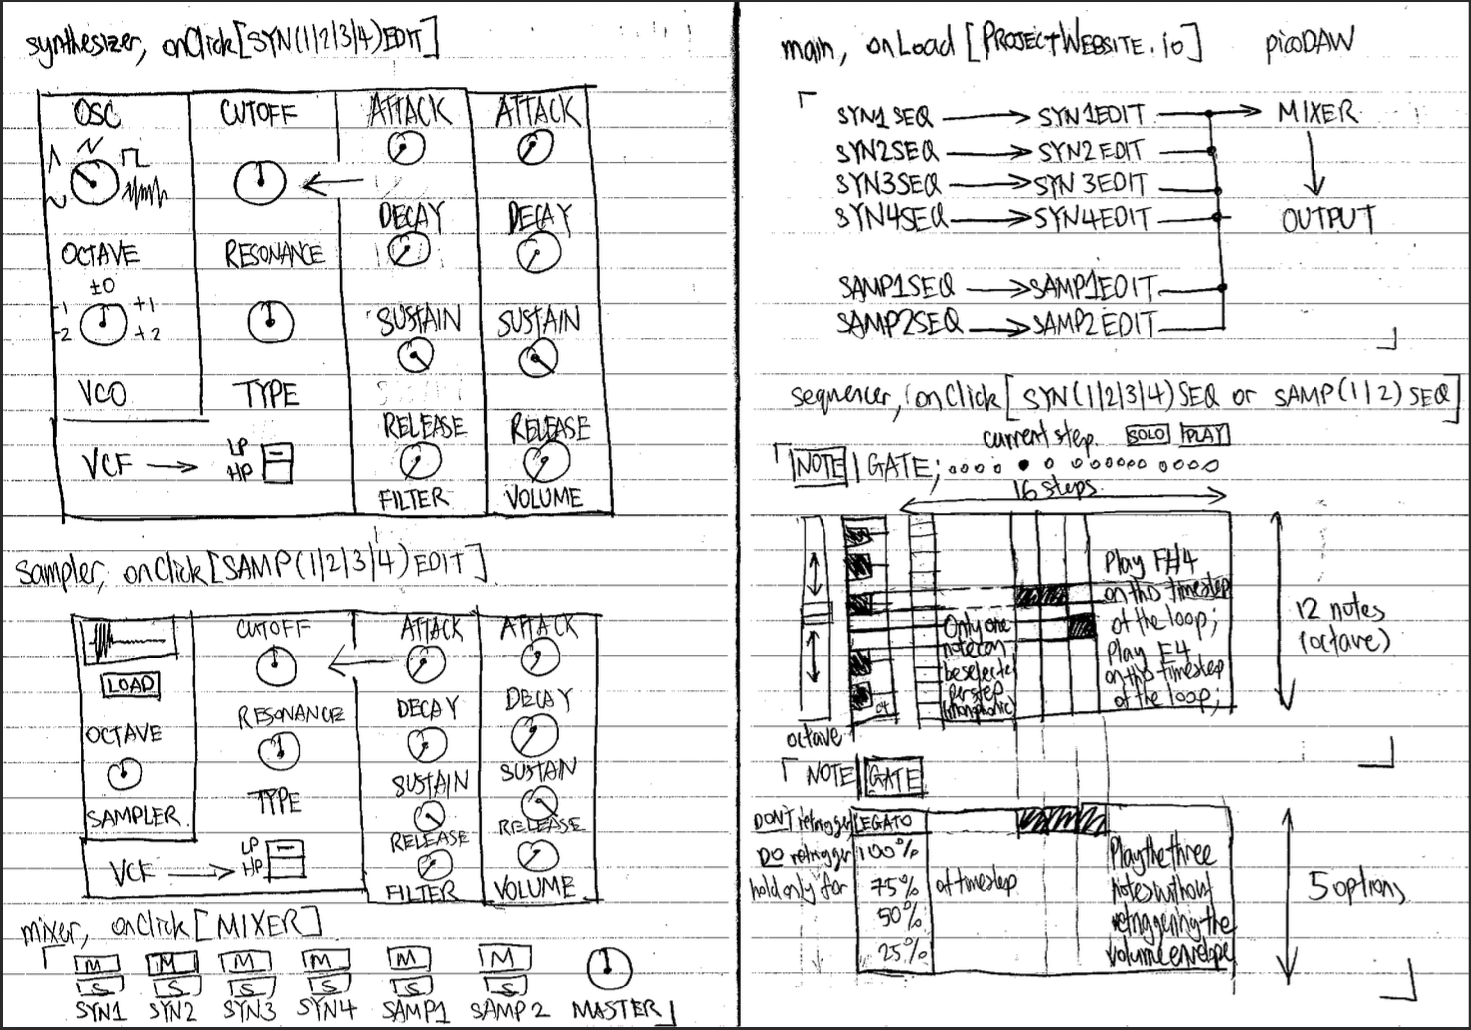
\includegraphics[width=0.9\columnwidth]{images/draft}

	\caption{Draft mockup of UI for picoDAW}
	\label{fig:draft}
\end{figure}
\noindent
See fig. \ref{fig:draft} for a draft mockup of picoDAW's UI.

Stretch goals, in case development goes easier than expected, include: (i) Pattern sequencer, enabling 
more expressive song creation; build multiple patterns, and then sequence them together to create a 
song. (ii) Two oscillators per synthesizer---instead of just one---making it easier to create chords, 
since the pitch of the second oscillator could be tuned to a specific note above or below the first 
oscillator. (iii) Volume control in mixer for each instrument, and basic effects---reverb, delay, and 
EQ---with routing done through the mixer. (iv) One 
LFO\footnote{\url{https://en.wikipedia.org/wiki/Low-frequency_oscillation}} per instrument; a triangle 
oscillator---of low frequency, proportional to \texttt{1/base\_timestep}---whose output can modulate 
the pitch of the instrument, providing basic FM synthesis. 


